\usetikzlibrary{calc}


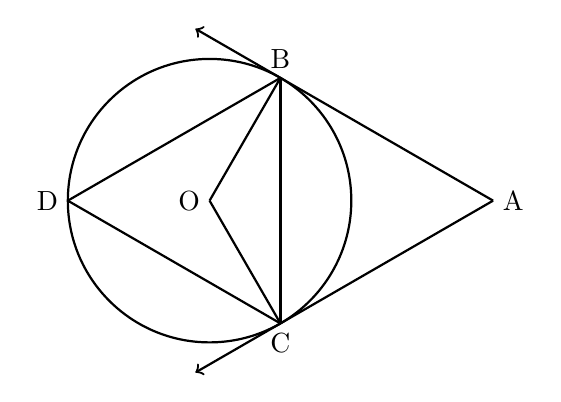
\begin{tikzpicture}[scale=1.2]
    % Define the center O and radius
    \coordinate (O) at (0,0);
    \def\radius{1.5}

    % Define point D on the left side of the circle
    \coordinate (D) at (-\radius, 0);

    % Define external point A
    % Placing A such that tangent points B and C are at 60 and -60 degrees
    % for nice proportions.
    % If B is at 60 deg, cos(60)=0.5, so A is at radius/0.5 = 3
    \coordinate (A) at (3, 0);

    % Define tangent points B and C
    \coordinate (B) at (60:\radius);
    \coordinate (C) at (-60:\radius);

    % Draw the circle
    \draw[thick] (O) circle (\radius);

    % Draw radii OB and OC
    \draw[thick] (O) -- (B);
    \draw[thick] (O) -- (C);

    % Draw chords BD, CD, and BC
    \draw[thick] (B) -- (D);
    \draw[thick] (C) -- (D);
    \draw[thick] (B) -- (C);

    % Draw tangent lines with arrows extending from A through B and C
    % Using calc library to extend the line past the tangent points
    \draw[thick, ->] (A) -- ($(A)!1.4!(B)$);
    \draw[thick, ->] (A) -- ($(A)!1.4!(C)$);

    % Add Labels
    \node[left] at (O) {O};
    \node[right] at (A) {A};
    \node[above] at (B) {B};
    \node[below] at (C) {C};
    \node[left] at (D) {D};

\end{tikzpicture}